\chapter{Detailed Design}
\label{chp:DetailedDesign}
This chapter documents the detailed design of the subsystems of the Ear-Monitor. The hardware and software sides are discussed separately. 

\section{Hardware}

A typical telemedicine configuration is used for the Ear-Monitor and its supporting system. Similar to that used in \cite{wang2010wearable} and \cite{prawiro2016integrated}. The ear-probe is the signal acquisition module, data is sent by means of a wireless transceiver to a device running supporting software and finally used data is stored for later access. Figure X illustrates the flow of information through the hardware set-up.

\begin{figure}[h]
\centering
\graphicspath{{figs/}}
%\def\svgwidth{200pt}
\input{figs/HardwareFlowchart.pdf_tex}
\caption{Flow of information in a typical telemedicine set-up}
\label{fig:HardwareFlowchart}
\end{figure}

This section documents the detailed design of each of the key parts of hardware found in the Ear-Monitor.

\subsection{Temperature sensor}
The non-contact, infrared TMP006 is selected to measure tympanic membrane temperature in the Ear-Monitor. Four wires are connected for power and communication. The package has eight solder balls for surface mounting on a PCB. A big challenge was to mount this micro-component. Various methods were tested. 

\medskip

First, a PCB was designed and manufactured. Mounting the TMP006 on this PCB proved to be problematic. Next, the device footprint and wire connection pads were etched into copper clad flexible PCB sheets. Solder paste and a heat gun was used to mount the TMP006. This method worked, but mounting proved to be unreliable, for connections were sometimes not made properly. Finally, it was decided to buy pre-mounted boards, cut away excess material and solder wires to the exposed tracks. This method was necessitated by the lack of advanced facilities to mount micro SMT components. The flex PCB method will be preferable when a SMT component placement system is available. Figure \ref{fig:TMP006_Breakout} shows the bought, pre-mounted boards and the cut-out component along with the four connections.

\begin{figure}[h]
   \centering
   \includegraphics[scale=0.8]{figs/TMP006_Breakout}
   \caption{TMP006 pre-mounted boards, cut-out and four connections}
   \label{fig:TMP006_Breakout}
\end{figure}

According to the TMP006 used guide, the sensor captures radiation form almost its entire 180\textdegree{} field of view, but the majority of the received signal comes from sources that are parallel to and precisely in front of the sensor. The final target object temperature is an integration of all the radiation signals captured across the field of view of the sensor.

\medskip

The user guide also states that the smaller the object is the closer it should be placed to the sensor to prevent other objects from entering the field of vision. It is suggested that a round object be placed at a distance of one halve of its radius from the sensor, relating to 1.75 mm in the case of the tympanic membrane. This is not nor practical or necessary in the case of the Ear-Monitor.  

\medskip

The goal is to place the sensor at least 5mm from the membrane. This will remove the risk of contact with the membrane, while still ensuring thermal radiation from the canal is detected. Energy from the ear canal self will inevitably be detected by the sensor, but it is assumed that the wall near the membrane is in thermal equilibrium with the membrane with in an acceptable margin.

\medskip

It is suggested that the sensor be placed at a distance no further than one-half of the radius of the target object. The minimum ear canal diameter of the test population will be 5mm, therefore the sensor must be placed 1.75 mm from the eardrum. Figure X shows the relationship between the target object size, distance from the sensor and percentage radiation captured from target object.

\medskip

Energy radiated or conducted between the PCB and the sensor can cause temperature calculation errors. To prevent this the sensor and PCB should be kept at the same temperature. The ear probe setup of this device is favourable for this task, for the PCB is very small and contains no other heat generating components. Also, the target object, tympanum, will stay at a constant temperature, so the sensor will experience no heat fluctuations. It will, however, be necessary to allow time for the sensor and PCB to reach thermal equilibrium once placed inside the ear canal, before accurate measurements can be taken.

\medskip

The TMP006 is placed in the tip of the ear probe. 